\documentclass{IOS-Book-Article}

\usepackage{cite}
\usepackage{mathptmx}

\usepackage[pdftex]{graphicx}
% declare the path(s) where your graphic files are
% \graphicspath{{../pdf/}{../jpeg/}}
% and their extensions so you won't have to specify these with
% every instance of \includegraphics
\DeclareGraphicsExtensions{.pdf,.jpeg,.png}

\usepackage{url}

% correct bad hyphenation here
\hyphenation{op-tical net-works semi-conduc-tor}

\newcommand{\psykal}{{PS}y{KA}l\ }

\def\hb{\hbox to 10.7 cm{}}

\begin{document}

\pagestyle{headings}
\def\thepage{}

\begin{frontmatter}              % The preamble begins here.

% can use linebreaks \\ within to get better formatting as desired
\title{Towards Performance Portability in Earth-System Modelling with GOcean.}

\markboth{}{November 2015\hb}
%\subtitle{Subtitle}

\author[A]{\fnms{A. R.} \snm{Porter}%
\thanks{Corresponding Author: Andrew Porter, STFC Daresbury Laboratory, Warrington, WA4 4AD, UK; E-mail:
andrew.porter@stfc.ac.uk.}},
\author[A]{\fnms{R. W.} \snm{Ford}},
\author[A]{\fnms{M.} \snm{Ashworth}},
\author[A]{\fnms{G. D.} \snm{Riley}}
and
\author[B]{\fnms{M.} \snm{Modani}}
\runningauthor{A.~R.~Porter et al.}
\address[A]{STFC Daresbury Laboratory, Warrington, WA4 4AD, UK}
\address[B]{IBM India}

\begin{abstract}
This paper presents a domain specific approach to performance
portability and the reduction of code complexity in finite-element and
finite-difference codes. This approach has been developed for the UK
Met Office's next generation atmospheric model which uses finite
elements on a quasi-unform grid, and has also been prototyped on two
finite difference Ocean model benchmarks, one of which is based on the
NEMO ocean model. We first outline our approach and then present
results for a range of compilers. These demonstrate that it is
possible to retain and potentially improve upon the performance of an
existing shallow water model while simultaneously reducing its code
complexity.
\end{abstract}

\begin{keyword}
Performance, Code-generation, Finite-difference
\end{keyword}

\end{frontmatter}
\markboth{November 2015\hb}{November 2015\hb}

%%%%%%%%%%%%%%%%%%%%%%%%%%%%%%%%%%%%%%%%%%%%%%%%%%%%%%%%%%%%%%%%%%%%
\section*{Introduction}

The challenge presented to the developers of scientific software by
the drive towards Exascale computing is considerable. With power
consumption becoming the overriding design constraint, CPU clock
speeds are falling and the complex, multi-purpose compute core is
being replaced by multiple, simpler cores. This philosophy can be seen
at work in the rise of so-called accelerator based machines in the Top
500 List~\cite{top500} of supercomputers: five of the top-ten machines
in the November 2014 list make use of Intel Xeon Phi's or NVIDIA
GPUs. Four of the remaining five machines in the top ten are IBM
BlueGene/Qs, the CPU of which has hardware support for running 64
threads.

Achieving good performance on large numbers of light-weight cores
requires exploiting as much parallelism in an application as possible
and this results in increased complexity in the programming models
that must be used. This in turn increases the burden of code
maintenance and code development, in part because two specialisms are
required: that of the scientific domain which a code is modelling
({\it e.g.} oceanography) and that of computational science. The
situation is currently complicated still further by the existence of
competing hardware technology; if one was to begin writing a major
scientific application today it is unclear whether one would target
GPU, Xeon Phi, traditional CPU, FPGA or something else entirely. This
is a problem because, generally speaking, these different technologies
require different programming approaches.

\section{The \psykal Approach}

The \psykal approach separates code into three layers; the Algorithm
layer, the PSy layer and the Kernel layer. While this approach is
general, we have applied it to Atmosphere and Ocean models written in
Fortran where domain decomposition is typically performed in the
latitude-longitude direction, leaving columns of elements on each
domain-decomposed partition.

The top layer, in terms of calling hierarchy, is the Algorithm
layer. This layer specifies the algorithm that the scientist would like
to perform (in terms of calls to kernel and infrastructure routines)
and logically operates on full fields. We say logically here as the
fields may be domain decomposed, however the algorithm layer is not
aware of this. It is the scientist's responsibility to write this
algorithm layer.

The bottom layer, in terms of calling hierarchy, is the Kernel
layer. The Kernel layer implements the science that the Algorithm
layer calls, as a set of subroutines. These kernels operate on local
fields (a set of elements, a single column of elements, or a set of
columns, depending on the kernel). Again the scientist is responsible
for writing this layer and there is no parallelism specified here, but
there is likely to be input from an HPC expert and/or some coding
rules to help make sure the kernels compile into efficient code.

The PSy layer sits in-between the Algorithm and Kernel layers and its
functional role is to link the algorithm calls to the associated
kernel subroutines. As the Algorithm layer works on logically global
fields and Kernel layer works on local fields, the PSy layer is
responsible for iterating over columns. It is also responsible for
including any required distributed-memory operations, such as halo
swaps and reductions.

As the PSy layer iterates over columns, the potential parallelism
within this iteration space can be optimised and parallelised. The PSy
layer can therefore be optimised for a particular hardware
architecture, such as multi-core, many-core, GPGPUs, or some
combination thereof with no change to the algorithm or kernel layer
code. This approach therefore offers the potential for portable
performance.

As an example, consider the following ``traditional'' code fragment:
\begin{verbatim}
!$OMP PARALLEL DO ...
do i = 1, nlat
  do j = 1, nlon
      do k = 1, levels
      a(k,j,i) = ...
      b(k,j,i) = ...
    end do
end do
end do
!$END OMP PARALLEL DO ...
\end{verbatim}
In the \psykal approach this code would be split into the {A}lgorithm
layer\ldots
\begin{verbatim}
call psy_...(a,b,...)
\end{verbatim}
PSy layer\ldots
\begin{verbatim}
subroutine psy_...(a,b,...)
  !$OMP PARALLEL DO ...
  do i = 1, nlat
    do j = 1, nlon
      call kern1(a,...)
      call kern2(b,...)
    end do
  end do
  !$END OMP PARALLEL DO
end subroutine psy_...
\end{verbatim}
and {K}ernel layer\ldots
\begin{verbatim}
subroutine kern1(a,...)
  do k = 1, levels
    a(k) = ...
  end do
end subroutine kern1
subroutine kern2(b,...)
  do k = 1, levels
    b(k) = ...
  end do
end subroutine kern2
\end{verbatim}

Therefore parallelism is encapsulated in the PSy layer and the
latitude-longitude iteration space can be parallelised in different
ways; the directives could be changed, the loops could be split, halo
calls could be added etc. None of these changes would require
modification to the Algorithm or Kernel layers.

One difference can be observed here. As kernels contain whole columns,
it is not possible to manually merge the ``k'' loops into one (which is
what was implemented in the original example code fragment). Such a
modification would have to be performed by the compiler, if the
compiler considered it appropriate.

Clearly the splitting of code into separate layers will have an effect
on performance. This overhead and how to get back to the performance
of the ``traditional'' code, and potentially improve on it, will be
discussed in the remainder of this paper.

\section{The `shallow' Program}

For the work described here we have used a benchmarking program that
solves the shallow-water equations on a bi-periodic plane, following
the finite-difference scheme introduced by Sadourny~\cite{sadourny75}.
This software was originally written in 1984 by Paul Swarztrauber of
the National Center for Atmospheric Research, US.  However, in common
with many scientific codes, it has subsequently undergone some sort of
evolutionary development with subsequent people making various changes
and optimising it for previous generations of hardware.  In describing
our work, we term the version of the Shallow program obtained at the
beginning of this project the `original' version.

Shallow is a very good test case for our purposes since the original
version is short (some 600 lines) and contained within a single source
file. This makes it relatively straightforward for a compiler to
optimise. Its performance is thus quite a demanding target for our
modified versions of the code to reproduce.

Since any real oceanographic computational model must output results,
we ensure that any \psykal version of Shallow retains the Input/Output
capability of the original. This aids in limiting the optimisations
that can be performed on the \psykal version to those that should also
be applicable to full oceanographic models. Note that although we
retain the I/O functionality, all of the results presented in this work
carefully exclude the effects of I/O since it is compute performance
that interests us here.

In order to maximise the flexibility (and thus potential for
optimisation) of the \psykal version of Shallow, we made the kernels
as fine-grained as possible. This resulted in eight
distinct kernels, each of which operated on a single field at a single
point (since we have chosen to use point-wise kernels). With a little
bit of tidying/re-structuring, we found it was possible to express the
contents of the main time-stepping loop as a single invoke (a call to
the PSy layer) and a call to the I/O system
(Figure~\ref{FIG_psykal_shallow_structure}). The single PSy-layer
routine then consists of applying each of the kernels to all of the
points on the model mesh requiring an update. In its basic,
unoptimised (`vanilla') form, this PSy-layer routine then contains a
doubly-nested loop around each kernel call, as indicated by the
pseudo-code in Figure~\ref{FIG_psykal_shallow_structure}.

\begin{figure}
\centering
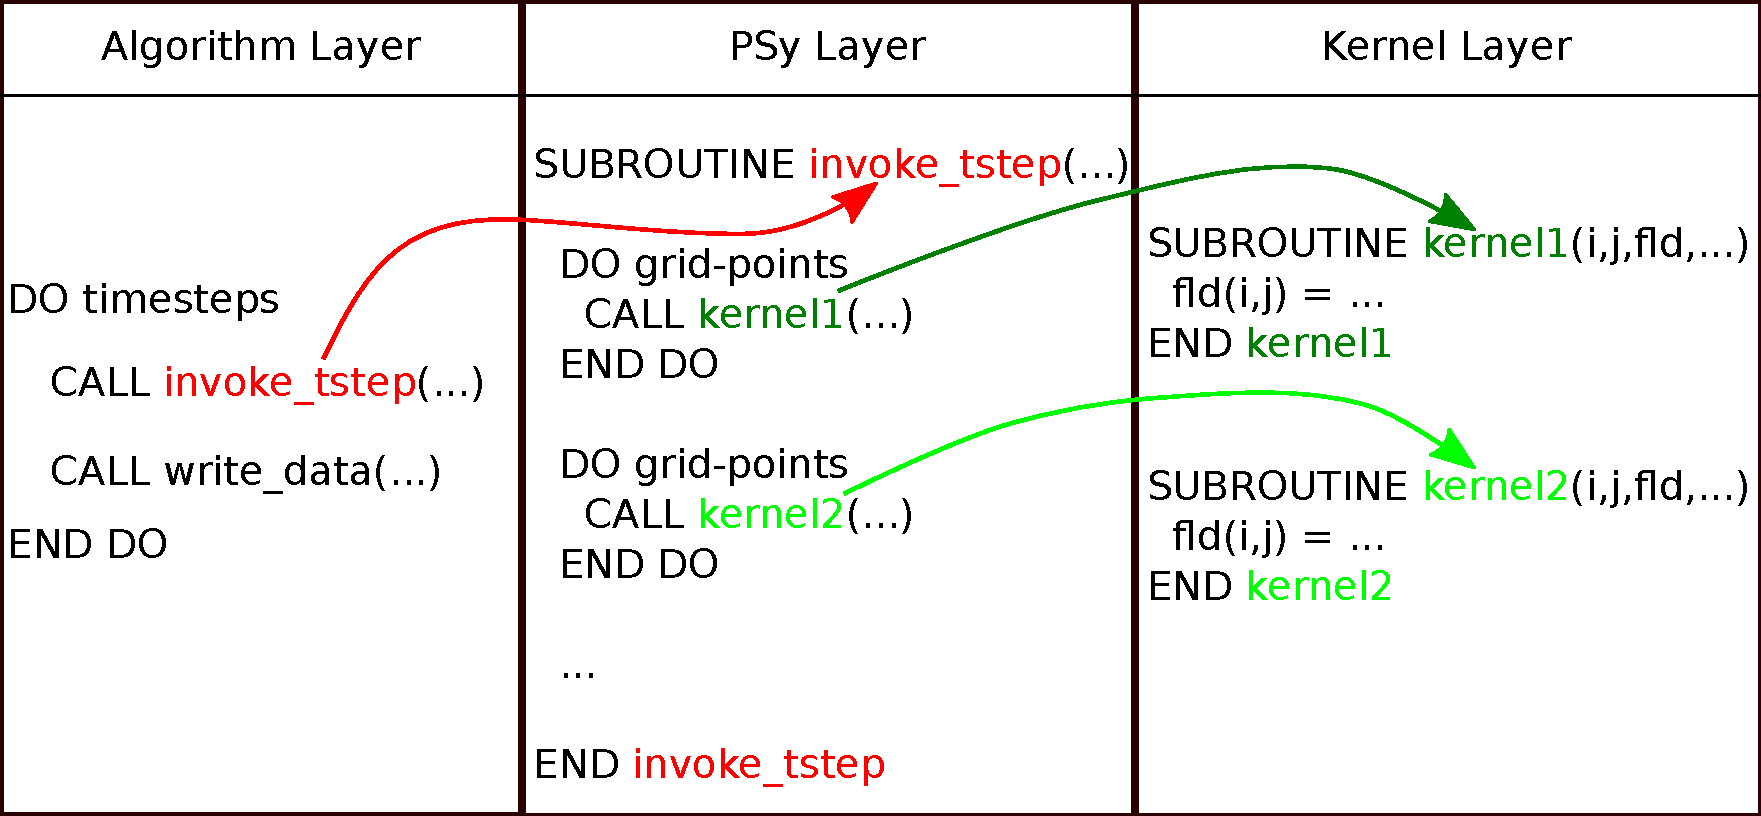
\includegraphics[width=85mm]{../psykal_shallow}
\caption{A schematic of the vanilla \psykal version of the shallow code.}
\label{FIG_psykal_shallow_structure}
\end{figure}

%%%%%%%%%%%%%%%%%%%%%%%%%%%%%%%%%%%%%%%%%%%%%%%%%%%%%%%%%%%%%%%%%%%%
\section{Methodology}

Our aim in this work is to achieve portable performance. Consequently,
we have performed tests with the hardware and compilers listed in
Table~\ref{TABLE_compilers}. Where a compiler is available on a given
piece of hardware, the version number used in this work is specified.

\begin{table}[!t]
% increase table row spacing, adjust to taste
\renewcommand{\arraystretch}{1.3}
\caption{The matrix of compilers and CPUs used in this work. The use
  of a compiler on a given CPU is indicated by the specification of
  the version of the compiler in the relevent element. The absence of an entry
  indicates that a compiler was not available/used on that CPU.}
\label{TABLE_compilers}
\centering
\begin{tabular}{|l|c|c|c|c|}
\hline
                 & \multicolumn{4}{c|}{Compiler}             \\
\hline
       CPU       & Gnu   & Intel       & Cray    & IBM     \\
\hline
Intel Haswell (E5-1620 v2)   & 4.8.2 & 14.0.0      &         & \\
Intel Ivy Bridge  (E5-2697 v2) & 4.9.1 & 14.0.1.106  & 8.3.3 & \\
IBM Power 8      &       &             &             & 14.1    \\
\hline
\end{tabular}
\end{table}

Before applying any code transformations, we benchmark the original
version of the code. We also benchmark the vanilla, unoptimised
version after it has been re-structured following the \psykal
approach. These two versions of the code effectively provide
approximate upper and lower bounds, respectively, on the performance
we expect to achieve.

Beginning with the vanilla \psykal version, we then apply a series of
code transformations while obeying the \psykal separation of concerns,
{\it i.e.} optimisation is restricted to the middle, {PS}y layer and
leaves the kernel and algorithm layers unchanged. The aim of these
optimisations is to recover, as much as is possible, the structure and
thus performance of the original version of the code.

We shall see that these optimisations do not always result in improved
performance. Whether or not they do so depends both on the compiler
and the problem size. We also emphasise that the aim of these
optimisations is to recover, as far as is possible, the structure of
the original version of the code. It may well be that transforming the
code into some other structure would result in better performance on a
particular architecture. However, exploring this optimisation space is
beyond the scope of the present work.

We explore the extent to which performance depends upon the problem
size by using square domains of dimension 64, 128, 256, 512 and
1024. This range allows us to investigate what happens when cache is
exhausted as well as giving us some insight into the decisions that
different compilers make when optimising the code.

%%%%%%%%%%%%%%%%%%%%%%%%%%%%%%%%%%%%%%%%%%%%%%%%%%%%%%%%%%%%%%%%%%%%
\section{Results}

In Figure~\ref{FIG_slowdown_summary} we plot the percentage difference
between the performance of the original and the (best) \psykal
versions of Shallow for each compiler/CPU combination.  It is clear
from this plot that the difference in the performance of the Gnu- and
Intel-compiled excutables on the Haswell system is due to the Gnu
compiler being unable to recover the performance achieved by the
original code. In contrast there is no such problem for the
Gnu-compiled executable on the Ivy Bridge system. We attribute this to
the more recent version of the compiler on the latter system (4.9.1 as
opposed to 4.8.2).

\begin{figure}[!t]
\centering
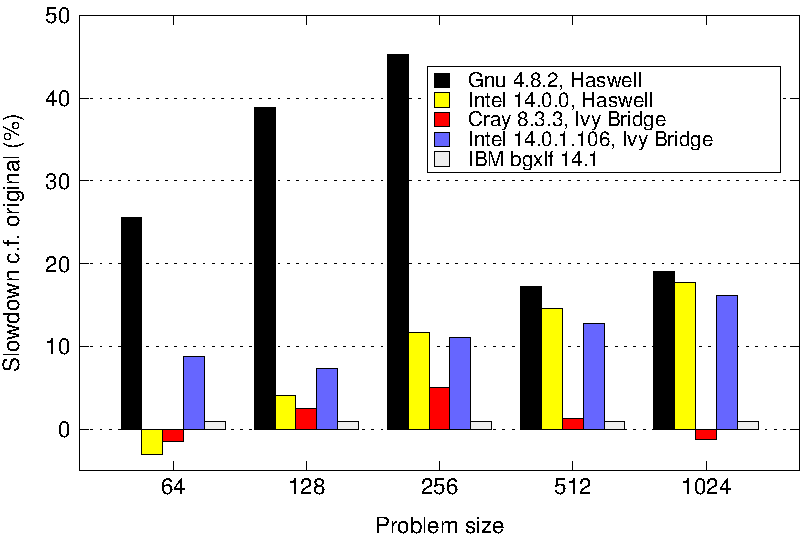
\includegraphics[width=90mm]{slowdown_summary}
\caption{Comparison of the performance of the best \psykal
version with that of the original version of the code. A negative value 
indicates that the \psykal version is faster than the original.}
\label{FIG_slowdown_summary}
\end{figure}

In fact, for the Gnu and Cray compilers on the Ivy Bridge system, the
\psykal version of shallow is never more than 2\% slower than the
original and in some cases is faster.  This demonstrates that we can
reliably recover the performance of the original version of the code,
despite the significant restructuring required by the \psykal
approach.

Having show that, in general, we can recover the performance of the
original code we next examine the code transformations that are required
(and must therefore be supported by the code-generation system).

%%%%%%%%%%%%%%%%%%%%%%%%%%%%%%%%%%%%%%%%%%%%%%%%%%%%%%%%%%%%%%%%%%%%
\section{Conclusions}

We have investigated the application of the \psykal separation of
concerns approach to the domain of finite-difference ocean
models. This approach enables the computational science (performance)
related aspects of a computer model to be kept separate from the
natural (oceanographic) science aspects. In this work we have shown
that the \psykal approach has the potential to at least maintain (if
not improve) performance while significantly improving code
structure/maintainability.

The application of code transformations/optimisations to the
middle/PSy layer is key to the performance of the \psykal version of a
code. In our approach this problem is tackled using the PSyclone
code-generation system which will be described in a future
publication.

%%%%%%%%%%%%%%%%%%%%%%%%%%%%%%%%%%%%%%%%%%%%%%%%%%%%%%%%%%%%%%%%%%%%
\section{Acknowledgments}

This work made use of the ARCHER UK National Supercomputing Service
(\url{http://www.archer.ac.uk}).

%%%%%%%%%%%%%%%%%%%%%%%%%%%%%%%%%%%%%%%%%%%%%%%%%%%%%%%%%%%%%%%%%%%%
\bibliography{../shallow_perf}{}
\bibliographystyle{unsrt}

\end{document}
